\documentclass[a4paper, 12pt]{article}

\usepackage{fontspec}
\usepackage[hidelinks]{hyperref}
\usepackage[catalan]{babel}
\usepackage{fullpage}
\usepackage{ragged2e}
\usepackage[a4paper, margin=2cm]{geometry}
\usepackage{graphicx}

\renewcommand*\contentsname{Índex}
\setlength\parindent{0pt}

\begin{document}
\title{Informe mecànic Projecte I}
\author{Marc Asenjo i Ponce de León \and
		Joan Marcè i Igual \and
		Iñigo Moreno i Caireta}
\date{\today}
\maketitle
\begin{center}
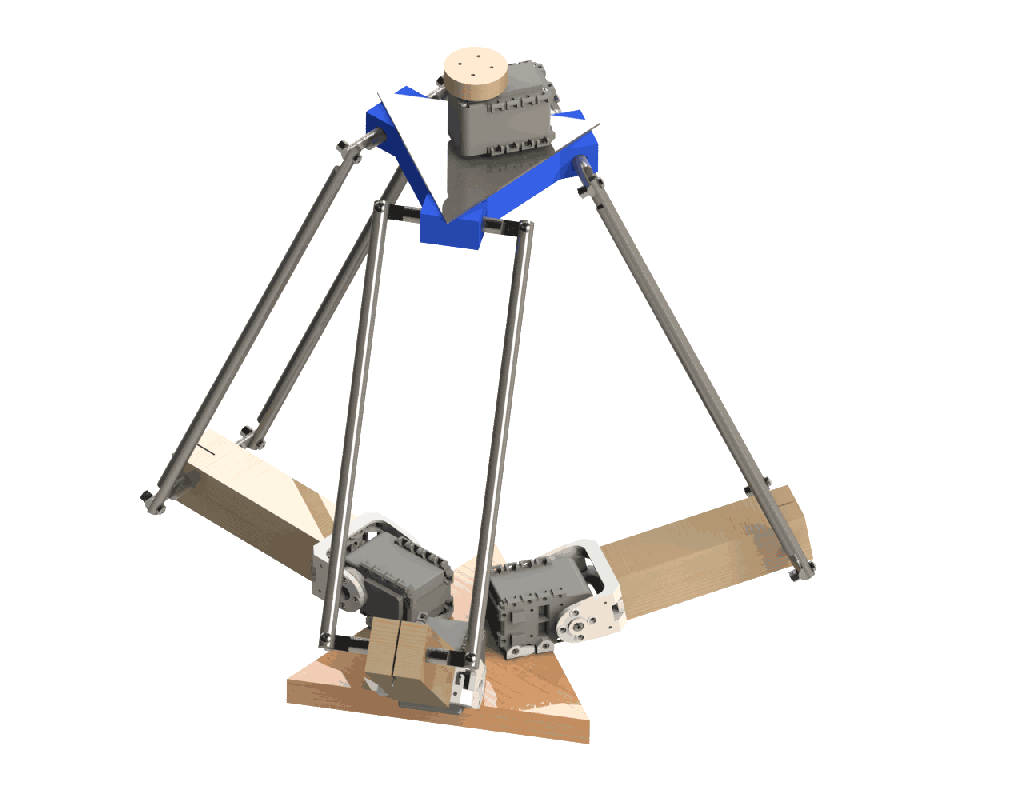
\includegraphics[width=0.5\textwidth]{./imgComp/logo}
\end{center}

\newpage
\tableofcontents{}

\newpage
\section{Ensamblatge general}

Aquest robot delta està format per quatre parts generals; els servos, els braços, els avantbraços i la pinça final. 

El robot consta de tres servos que permetran el posicionament de la pinça; cada servomotor té acoblat un braç que es mou junt amb l'eix d'aquest. A més a més, els
braços estan units mitjançant un eix amb l'avantbraç. Tots els avantbraços arriben a unir-se a la peça final que és la pinça permetent així que el moviment dels tres servos determini un punt a l'espai en el qual posicionar la pinça amb tres graus de llibertat de translació.

\begin{figure}[h!]
\centering
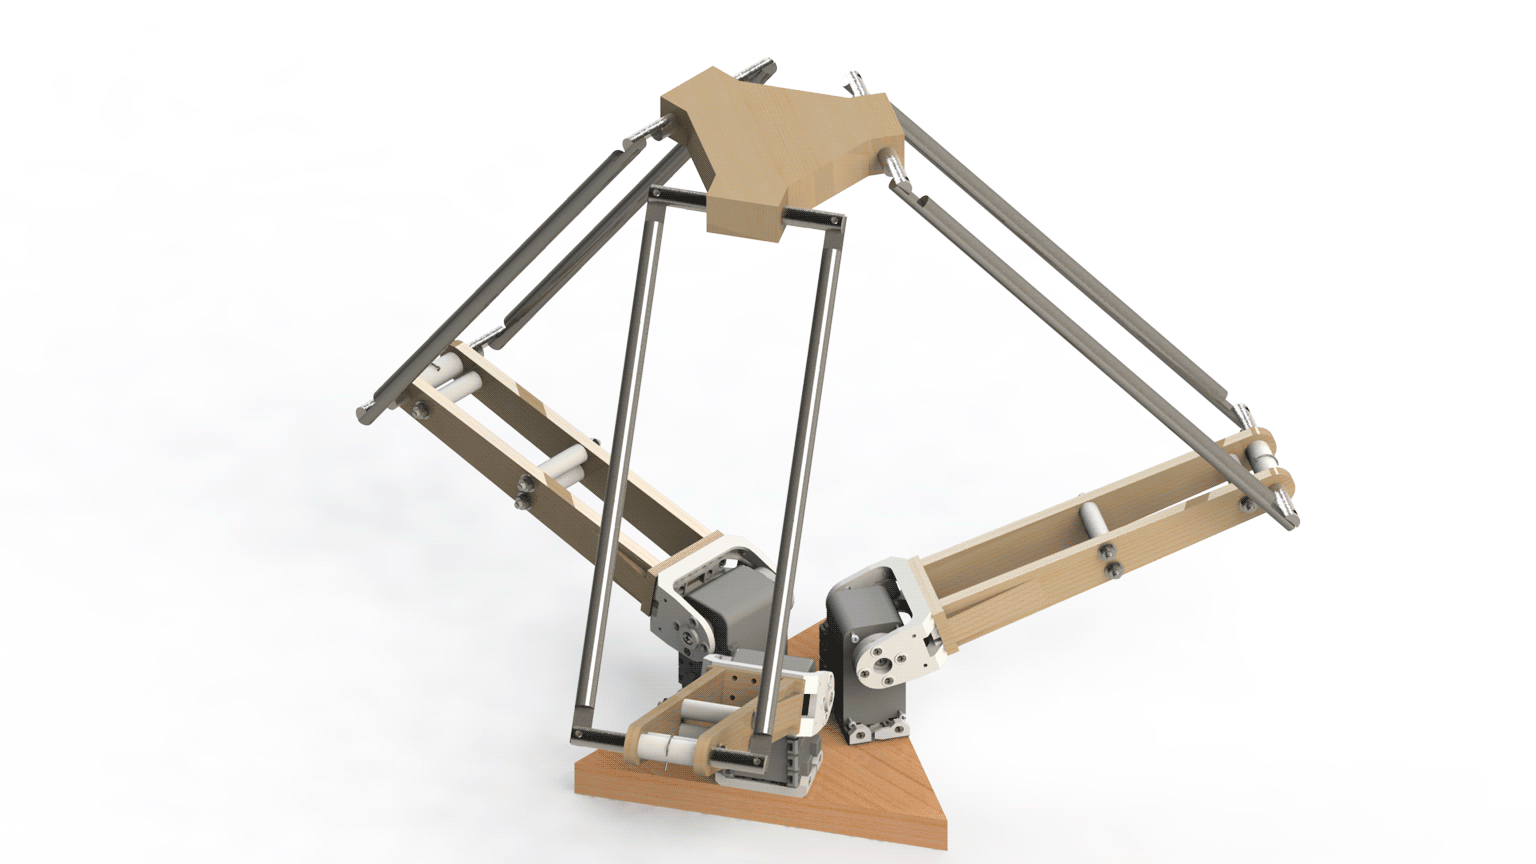
\includegraphics[width=10cm]{./imgComp/general}
\caption{Ensamblatge general}
\end{figure}



\newpage
\section{Servomotors}
Els servomotors permeten el posicionament específic d'un eix a un cert angle. N'hi ha tres. S'utilitza el model AX-12 de dynamixel. 

A part dels servos també s'han utilitzat els accessoris \emph{FP04-F2 i FP04-F3}. Per tal de facilitar l'ancoratge entre el servomotor i les diferents peces.

\begin{figure}[h!]
\centering
\begin{minipage}[b]{0.45\linewidth}
\centering
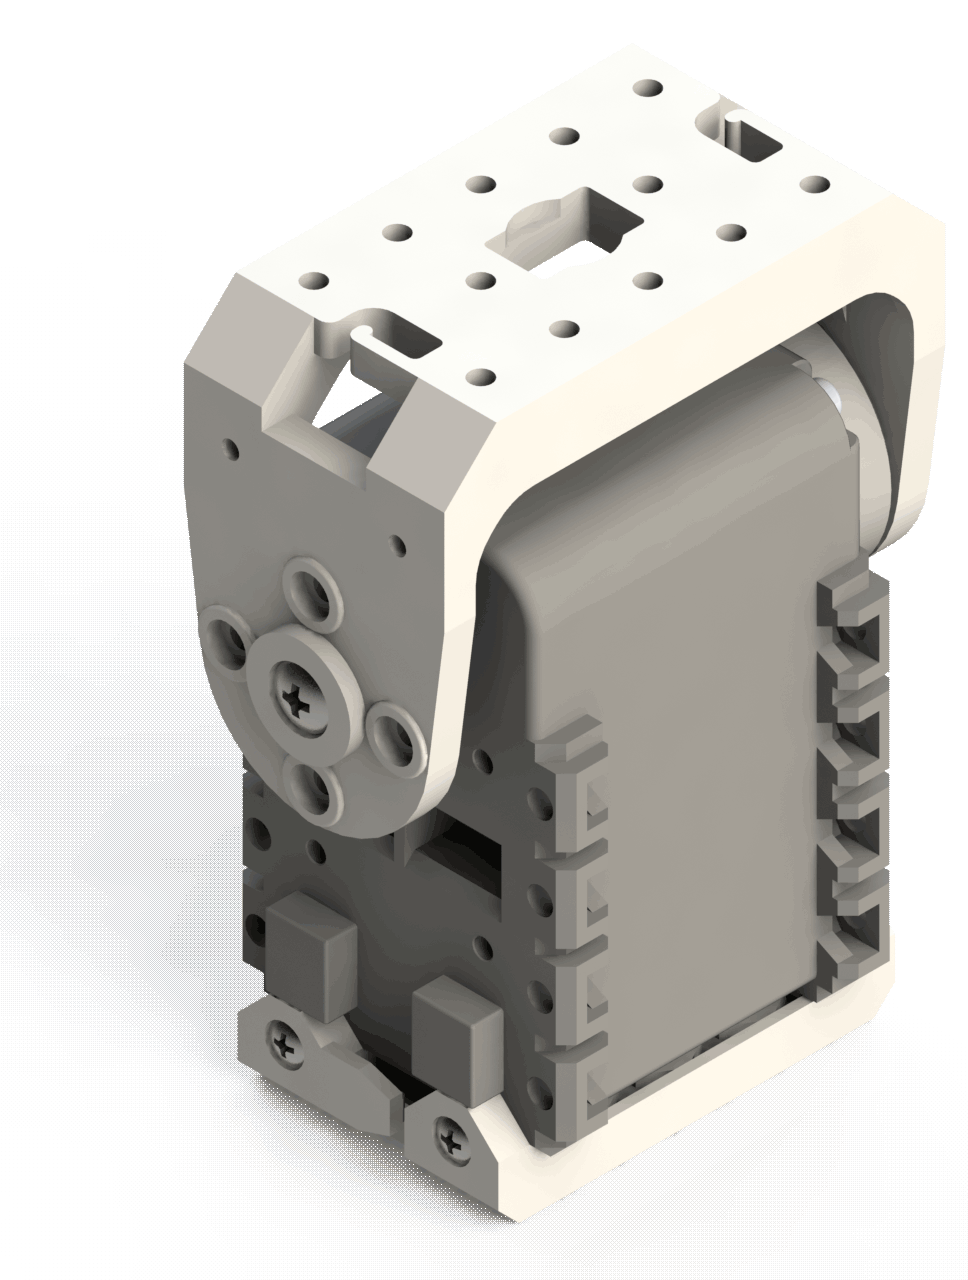
\includegraphics[width=6cm]{./imgComp/servo}
\caption{Imatge 3D del servomotor}
\end{minipage}
\begin{minipage}[b]{0.45\linewidth}
\centering
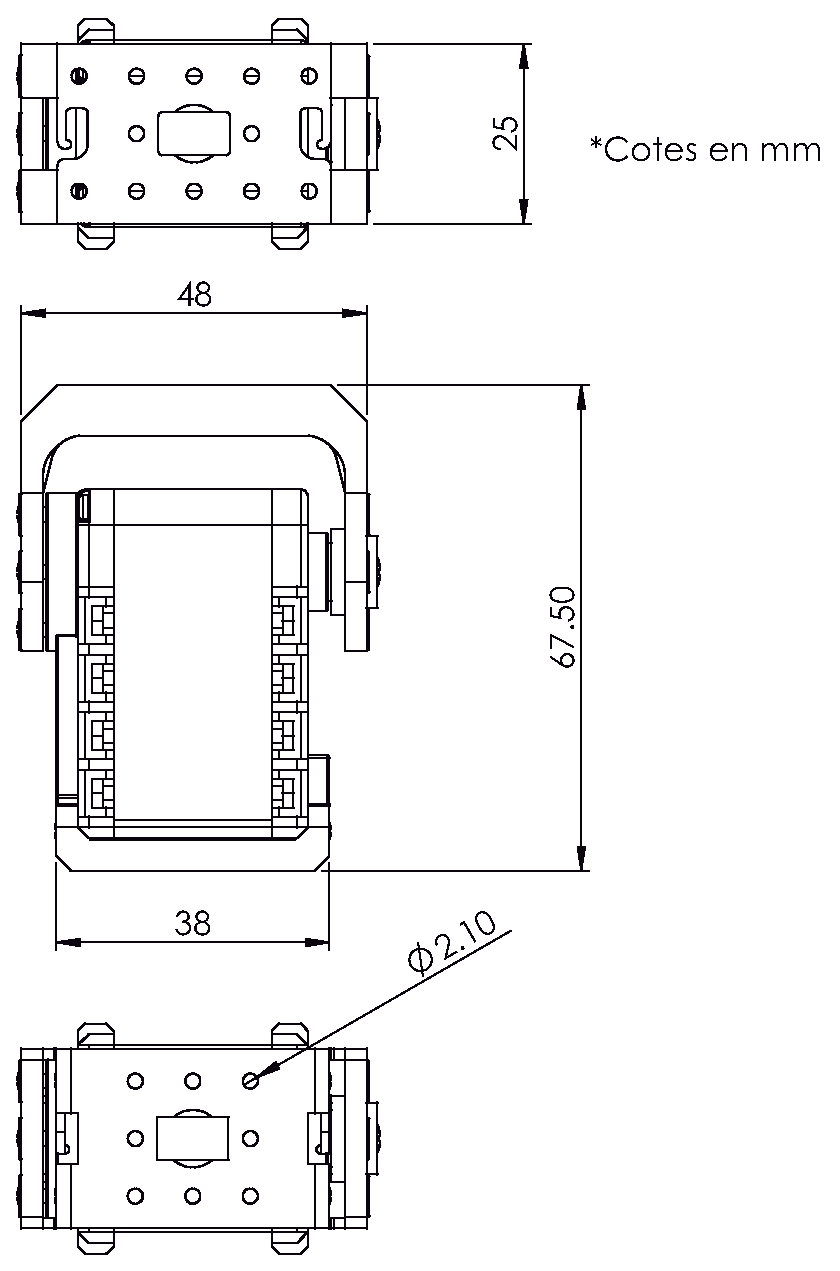
\includegraphics[width=7cm]{./sketch/servo}
\caption{Plànol del servomotor amb els accessoris}
\end{minipage}
\end{figure}


\newpage
\section{Braç}
Es recolza en els servomotors i principalment està fet de fusta. La part estructural és tota de fusta i està tota enganxada amb cola i després hi ha tres estabilitzadors que eviten vibracions innecessàries a la part del braç més propera a l'eix. 

\begin{figure}[h!]
\begin{minipage}[b]{0.45\linewidth}
\centering
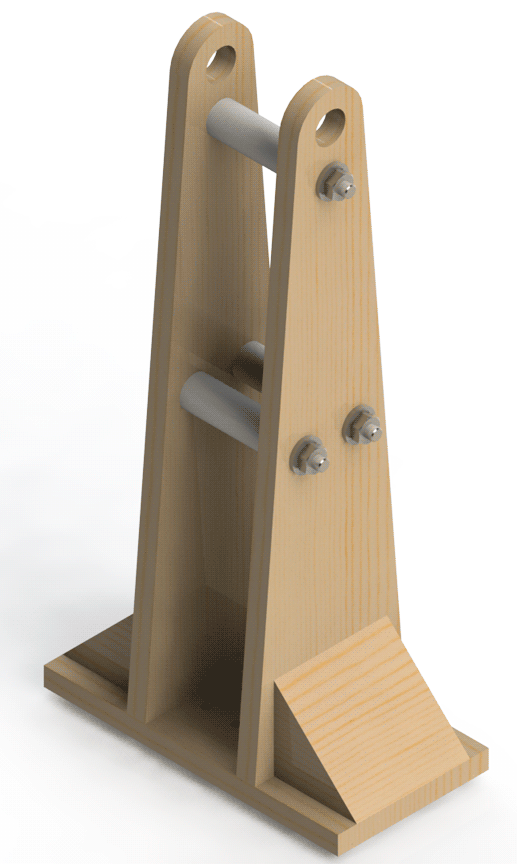
\includegraphics[height=6.5cm]{./imgComp/brac}
\caption{Braç muntat}
\end{minipage}
\begin{minipage}[b]{0.45\linewidth}
\centering
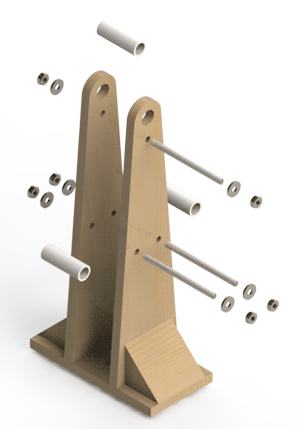
\includegraphics[height=6.5cm]{./imgComp/brac_expl}
\caption{Muntatge del braç}
\end{minipage}
\end{figure}

\subsection{Estructura}
L'estructura està feta amb llistons de fusta. S'ha utilitzat un llistó de 45º d'inclinació per la part de suport que es troba entre la base i la columna vertical i per a fer tant la base com les columnes verticals s'ha utilitzat un llistó de 5 mm de gruix que s'ha tallat perquè tingui la forma desitjada. 

La raó per la que s'ha escollit fer-ho amb fusta és per poder fer-hi forats i talls amb relativa facilitat ja que la fusta és fàcil de treballar; també el reduït cost econòmic d'aquesta ha motivat escollir aquest material.
\begin{figure}[h!]
\begin{minipage}[b]{.45\linewidth}
\centering
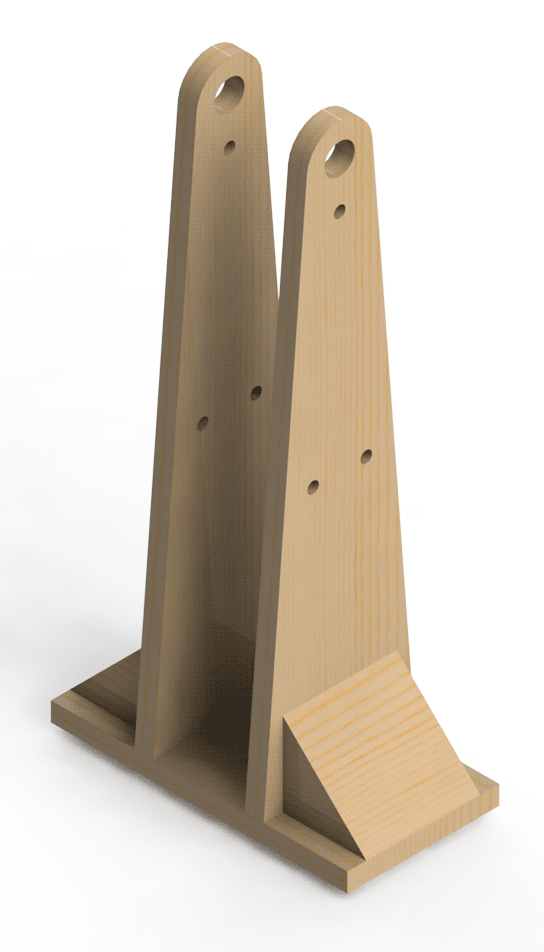
\includegraphics[height=7cm]{./imgComp/estructura}
\caption{Estructura del braç}
\end{minipage}
\begin{minipage}[b]{.45\linewidth}
\centering
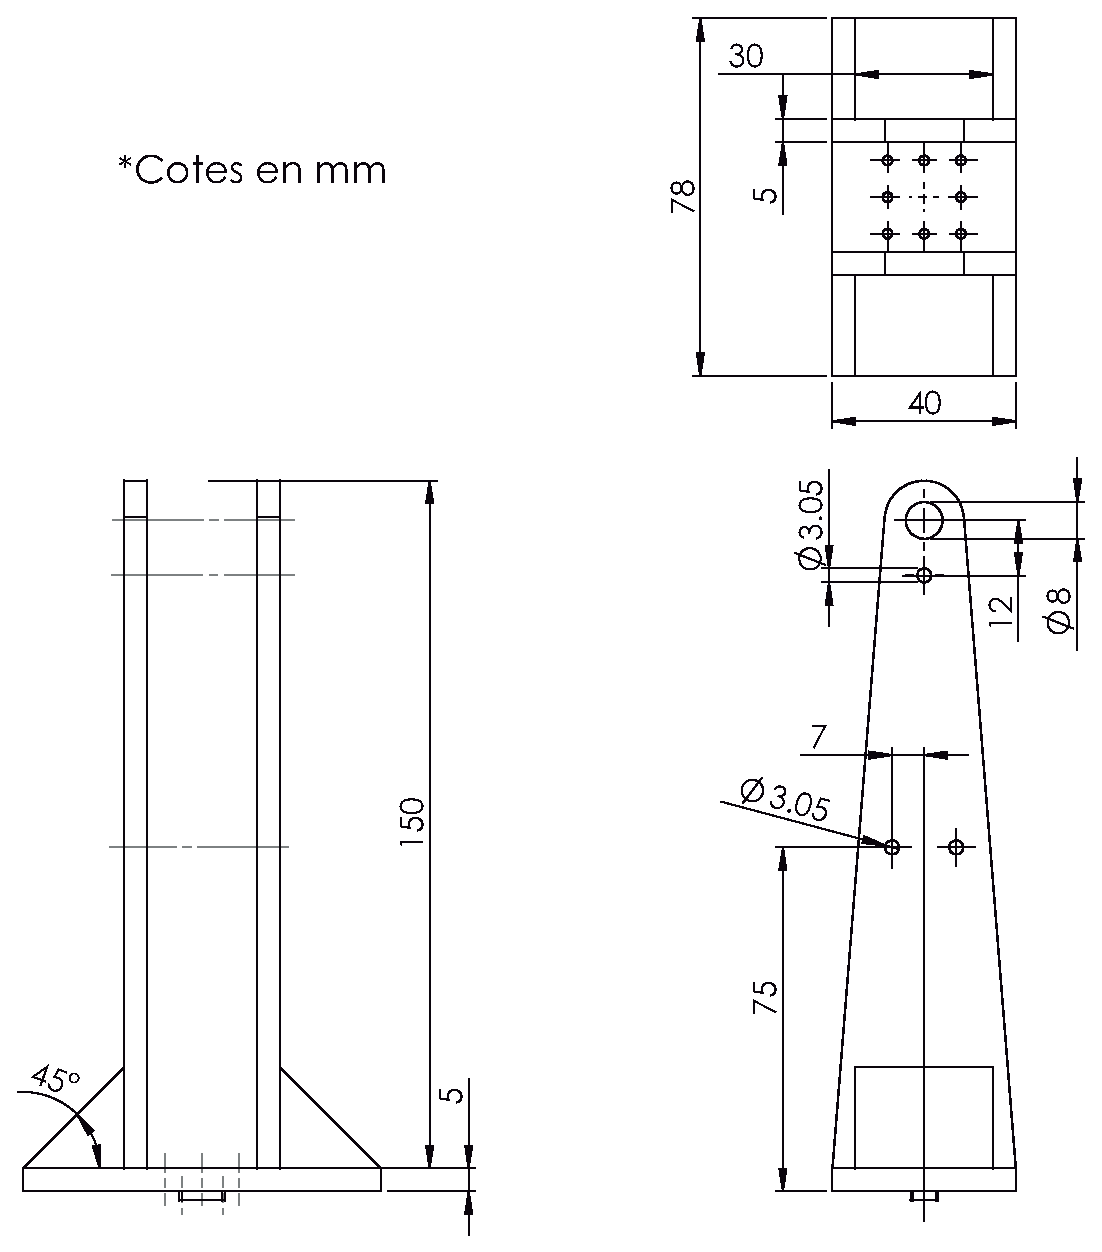
\includegraphics[height=8.2cm]{./sketch/estructura}
\caption{Plànol de les mides del braç}
\end{minipage}
\end{figure}

\subsection{Estabilitzador}
L'estabilitzador s'utilitza per tal que l'estructura de fusta no vibri ni es deformi degut al moviment del robot. 
És un conjunt de peces que està format per:
\begin{itemize}
\item Una barra roscada de M3 i 45 mm de llargada

\item Un tub de plàstic de 6 mm de diàmetre interior i 8 mm de diàmetre exterior de 24 mm de llargada

\item Dues volanderes

\item Dues femelles M3
\end{itemize}

El tub de plàstic es situa entre les dues fustes verticals de l'estructura del braç i per dins hi va la barra roscada. A fora es col·loquen les femelles i les volanderes de manera que permeten prémer les dues fustes contra el tub de plàstic forçant així que la distància entre les dues fustes sigui constant.

\begin{figure}[h!]
\begin{minipage}[b]{0.45\linewidth}
\centering
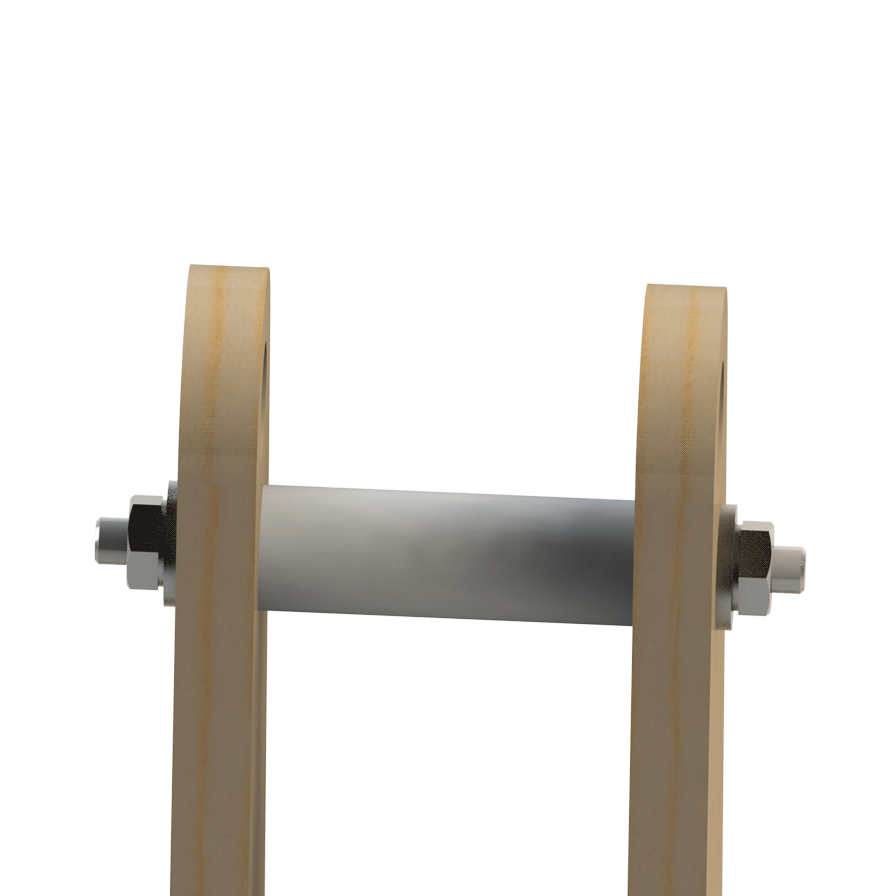
\includegraphics[height=5cm]{./imgComp/estab}
\caption{Estabilitzador muntat}
\end{minipage}
\begin{minipage}[b]{0.45\linewidth}
\centering
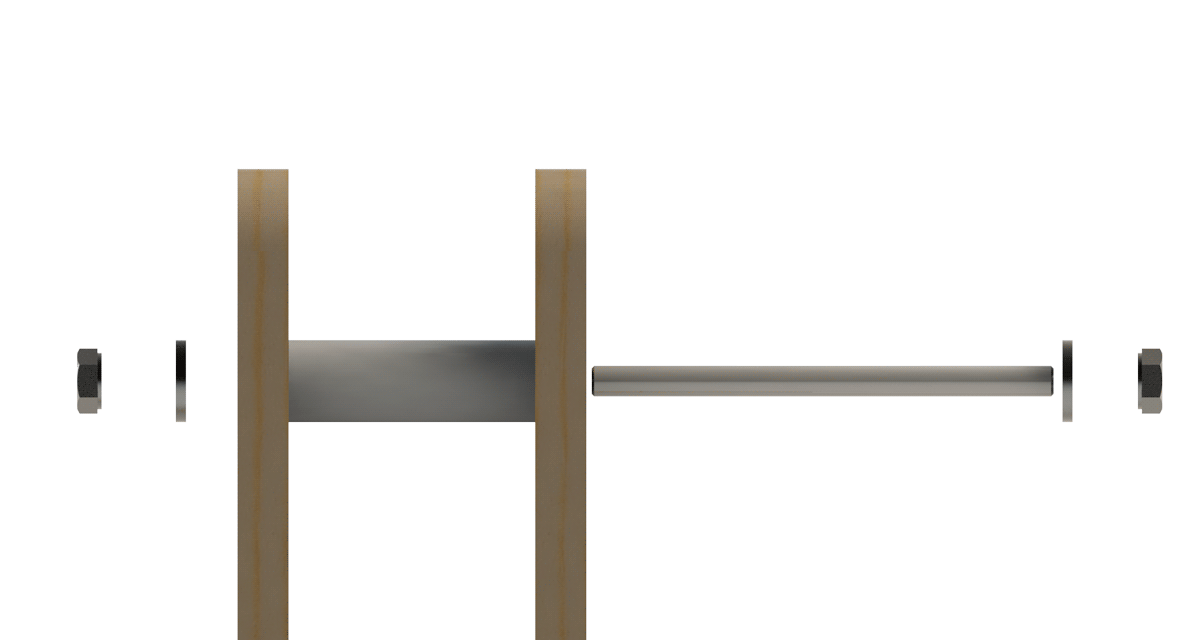
\includegraphics[height=5cm]{./imgComp/estab_expl}
\caption{Muntatge estabilitzador}
\end{minipage}
\end{figure}

\newpage
\section{Avantbraç}

\begin{figure}[h!]
\begin{minipage}[b]{.45\linewidth}
\centering
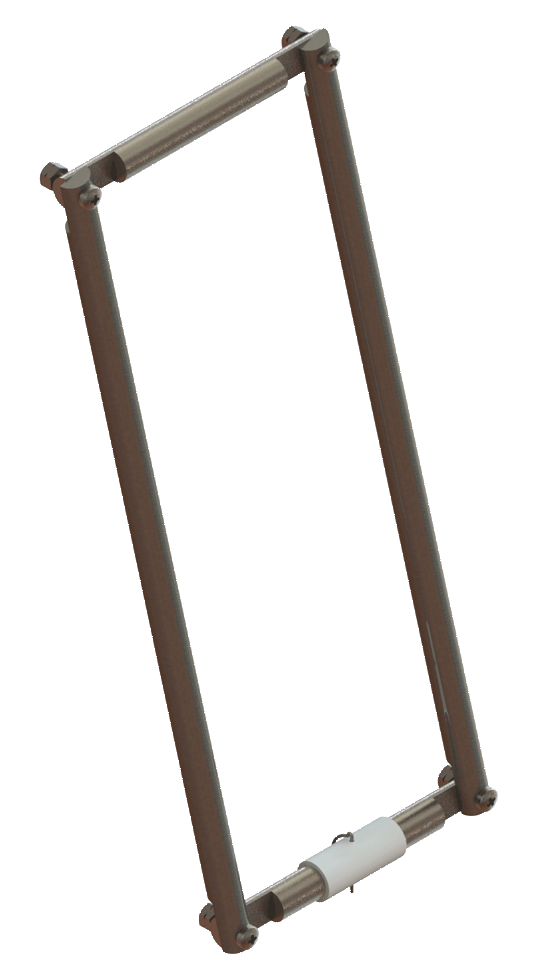
\includegraphics[height=7cm]{./imgComp/avant}
\caption{Avantbraç muntat}
\end{minipage}
\begin{minipage}[b]{.45\linewidth}
\centering
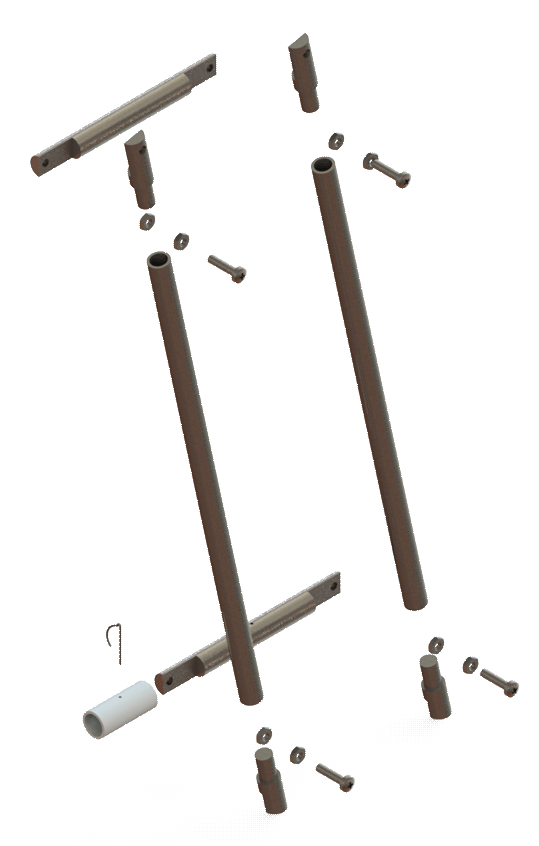
\includegraphics[height=7cm]{./imgComp/avant_expl}
\caption{Muntatge avantbraç}
\end{minipage}
\end{figure}

\subsection{Vara}

\subsection{Eix}

\subsection{Eix Pinça}

\subsection{Unió}

\newpage
\section{Pinça}

\end{document}